% Chapter Template

% Main chapter title
\chapter{Results}

% Short version of the title for the header
\chaptermark{Results}

% Chapter Label
\label{chap:results}

This chapter presents the experimental results of our tokenizer adaptation method. We first report benchmark results across downstream tasks, followed by a qualitative analysis of model outputs in the target language. Additionally, we introduce a custom efficiency metric (\S\ref{sec:gen_efficiency}) to assess the impact of tokenizer modifications on token usage during generation.


\section{Quantitative Results}

The goal of the quantitative evaluation is to determine whether vocabulary expansion affects a model’s ability to understand and generate Portuguese text. We assess two complementary dimensions:  
(i) \textbf{accuracy}, measured through benchmark tasks that test reasoning and completion, and  
(ii) \textbf{efficiency}, measured through our custom FertilityBoost metric that captures tokenization economy.  

Together, these results allow us to quantify both the stability of downstream performance and the potential cost savings in token usage introduced by tokenizer adaptation.


\subsection{Benchmark Accuracy}
All evaluations follow the benchmark-specific protocols described in Chapter~\ref{Section3}. For clarity:

\begin{itemize}
    \item \textbf{CalamePT:} Accuracy is measured as the proportion of correctly predicted final words in incomplete Portuguese phrases.
    \item \textbf{SuperGluePTPT (BoolQ-PT):} Accuracy is measured as the proportion of correct yes/no answers in the binary classification task.
\end{itemize}

We compare baseline models against variants adapted with (i) added tokens only and (ii) added tokens followed by lightweight embedding training introduced in (\S\ref{sec:embedding_finetune}). 


Table~\ref{tab:benchmark-results} reports the performance of the three evaluated models (\texttt{SmolLM2-135M}, \texttt{SmolLM3-3B}, and \texttt{Qwen2.5-1.5B-Instruct}) under different adaptation strategies.

\begin{table}[H]
\centering
\begin{tabular}{lcccc}
\hline
\textbf{Model} & \textbf{New Tokens} & \textbf{Type} & \textbf{CalamePT (\%)} & \textbf{SuperGluePTPT (\%)} \\
\hline
SmolLM2-135M & 0     & Baseline      & 13.54 & 1.47 \\
SmolLM2-135M & 1000  & No Training   & 13.54 & 1.47 \\
SmolLM2-135M & 1000  & With Training & 13.54 & 1.47 \\
SmolLM2-135M & 5000  & No Training   & 13.54 & 1.51 \\
SmolLM2-135M & 5000  & With Training & 13.54 & 1.51 \\
SmolLM2-135M & 7500  & No Training   & 13.54 & 1.51 \\
SmolLM2-135M & 7500  & With Training & 13.54 & 1.51 \\
\hline
SmolLM3-3B   & 0     & Baseline      & 58.53 & 49.69 \\
SmolLM3-3B   & 1000  & No Training   & 58.53 & 49.69 \\
SmolLM3-3B   & 1000  & With Training & 58.53 & 49.69 \\
SmolLM3-3B   & 5000  & No Training   & 58.53 & 49.69 \\
SmolLM3-3B   & 5000  & With Training & 58.53 & 49.69 \\
SmolLM3-3B   & 7500  & No Training   & 58.53 & 49.69 \\
SmolLM3-3B   & 7500  & With Training & 58.53 & 49.69 \\
\hline
Qwen2.5-1.5B-Instruct & 0     & Baseline      & 49.61 & 40.24 \\
Qwen2.5-1.5B-Instruct & 1000  & No Training   & 49.61 & 39.86 \\
Qwen2.5-1.5B-Instruct & 1000  & With Training & 49.61 & 39.79 \\
Qwen2.5-1.5B-Instruct & 5000  & No Training   & 49.61 & 40.28 \\
Qwen2.5-1.5B-Instruct & 5000  & With Training & 49.61 & 40.21 \\
Qwen2.5-1.5B-Instruct & 7500  & No Training   & 49.57 & 40.14 \\
Qwen2.5-1.5B-Instruct & 7500  & With Training & 49.57 & 40.06 \\
\hline
\end{tabular}
\caption{Performance on Portuguese Benchmarks (CalamePT and SuperGluePTPT)}
\label{tab:benchmark-results}
\end{table}

Overall, benchmark accuracy remains stable across most configurations. Minor fluctuations (≤0.5\%) suggest that vocabulary expansion has little effect on high-level reasoning (SuperGluePTPT) or text completion (CalamePT) without more extensive training.


\subsection{Generation Efficiency}
\label{sec:gen_efficiency}

While benchmark accuracy measures correctness, generation efficiency highlights how economically a model uses tokens to represent words. This matters because inefficient tokenization increases sequence length, computation time, and inference costs. To capture this, we report the metrics\textbf{FertilityOutput} (\S\ref{subsec:fertility_output}) and \textbf{FertilityBoost} (\S\ref{subsec:fertility_boost}) for each configuration.

Table~\ref{tab:fertility_results} summarizes the tokenization efficiency results. We report \textbf{FertilityOutput} (average tokens per Portuguese word) and relative \textbf{FertilityBoost} compared to baseline.

\begin{table}[H]
\centering
\begin{tabular}{lcccc}
\hline
\textbf{Model} & \textbf{New Tokens} & \textbf{Type} & \textbf{FertilityOutput} & \textbf{FertilityBoost\footnote{Ran with Temperature=0.8 over 10 runs}} \\
\toprule
HuggingFaceTB/SmolLM2-135M &                  0 &       Baseline &         3.07 &             - \\
HuggingFaceTB/SmolLM2-135M &               1000 &    No Training &         3.24 &   $5.07\% \pm 0.05\%$ \\
HuggingFaceTB/SmolLM2-135M &               1000 &  With Training &         3.30 &   $5.05\% \pm 0.06\%$ \\
HuggingFaceTB/SmolLM2-135M &               5000 &    No Training &         2.76 &  $12.88\% \pm 0.04\%$ \\
HuggingFaceTB/SmolLM2-135M &               5000 &  With Training &         2.79 &  $12.94\% \pm 0.11\%$ \\
HuggingFaceTB/SmolLM2-135M &               7500 &    No Training &         2.83 &  $16.03\% \pm 0.11\%$ \\
HuggingFaceTB/SmolLM2-135M &               7500 &  With Training &         2.86 &  $15.99\% \pm 0.12\%$ \\
\midrule
HuggingFaceTB/SmolLM3-3B   &                  0 &       Baseline &         2.00 &             - \\
HuggingFaceTB/SmolLM3-3B   &               1000 &    No Training &         2.11 &   $0.22\% \pm 0.01\%$ \\
HuggingFaceTB/SmolLM3-3B   &               1000 &  With Training &         2.11 &   $0.22\% \pm 0.01\%$ \\
HuggingFaceTB/SmolLM3-3B   &               5000 &    No Training &         2.05 &   $0.87\% \pm 0.04\%$ \\
HuggingFaceTB/SmolLM3-3B   &               5000 &  With Training &         2.04 &   $0.84\% \pm 0.06\%$ \\
HuggingFaceTB/SmolLM3-3B   &               7500 &    No Training &         2.02 &   $1.05\% \pm 0.04\%$ \\
HuggingFaceTB/SmolLM3-3B   &               7500 &  With Training &         2.03 &   $1.06\% \pm 0.04\%$ \\
\midrule
Qwen/Qwen2.5-1.5B-Instruct &                  0 &       Baseline &         1.74 &             - \\
Qwen/Qwen2.5-1.5B-Instruct &               1000 &    No Training &         2.19 &   $0.63\% \pm 0.02\%$ \\
Qwen/Qwen2.5-1.5B-Instruct &               1000 &  With Training &         2.21 &   $0.62\% \pm 0.02\%$ \\
Qwen/Qwen2.5-1.5B-Instruct &               5000 &    No Training &         2.19 &   $2.09\% \pm 0.04\%$ \\
Qwen/Qwen2.5-1.5B-Instruct &               5000 &  With Training &         2.26 &   $2.12\% \pm 0.05\%$ \\
Qwen/Qwen2.5-1.5B-Instruct &               7500 &    No Training &         2.19 &   $2.56\% \pm 0.04\%$ \\
Qwen/Qwen2.5-1.5B-Instruct &               7500 &  With Training &         2.17 &   $2.52\% \pm 0.04\%$ \\
\bottomrule
\end{tabular}
\caption{Tokenization Efficiency}
\label{tab:fertility_results}
\end{table}

The results show clear differences across model scales:
\begin{itemize}
    \item \textbf{SmolLM2-135M} benefited significantly from new tokens, with up to a \textbf{16\% improvement} in tokenization efficiency.
    \item \textbf{SmolLM3-3B} showed only marginal gains (~1\%), suggesting diminishing returns at larger model sizes.
    \item \textbf{Qwen2.5-1.5B-Instruct} exhibited small positive boosts (≤2.5\%), but also incurred higher FertilityOutput overall, reflecting tokenization instability.
\end{itemize}

These findings suggest that vocabulary adaptation is particularly useful for small-scale models, while larger multilingual models are less sensitive to such modifications.




\subsection{New Token Rank Distribution}

To better understand whether the newly introduced tokens are likely to be selected during generation, we conducted a rank distribution analysis: 
\begin{enumerate}
    \item Select instances from Portuguese datasets where the newly added tokens occur;  
    \item Prompt the model up to the point where the new token should be generated;  
    \item Compute the rank and logits of both:
        \begin{enumerate}
            \item The original sub-token sequence (e.g., ``cas'' in ``cas+inha'')
            \item The corresponding new token (e.g., ``casinha''); 
        \end{enumerate}
    \item Repeat this for all occurrences of new tokens.  
\end{enumerate}


This analysis provides insight into whether the adapted model assigns a higher probability mass (i.e. lower rank) to the new tokens compared to the original decomposition.  

Figure~\ref{fig:new_token_rank} summarizes the scores obtained across all evaluated generation while Figure~\ref{fig:violin_rank_dist} showcases the distribution of the difference $new\_token\_rank - old\_token\_rank$. We observe that, in many cases, the new token achieves a higher score than the original sequence, suggesting that the model internally recognizes the utility of these merged units. This effect is especially relevant under stochastic decoding strategies (\textit{temperature} $>0$), where alternative tokens can be sampled.  

\begin{figure}[H]
    \centering
    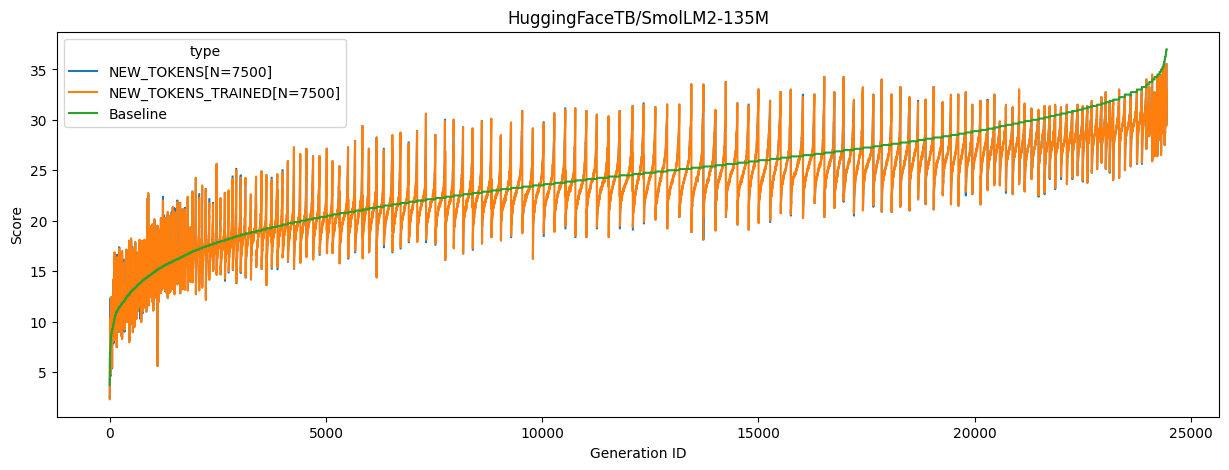
\includegraphics[width=0.75\textwidth]{Figures/rank_distribution_smolLM2.png}
    \caption{Score comparison between original sub-token sequences and newly introduced tokens. Higher ranks indicate higher model preference.}
    \label{fig:new_token_rank}
\end{figure}

\begin{figure}[H]
    \centering
    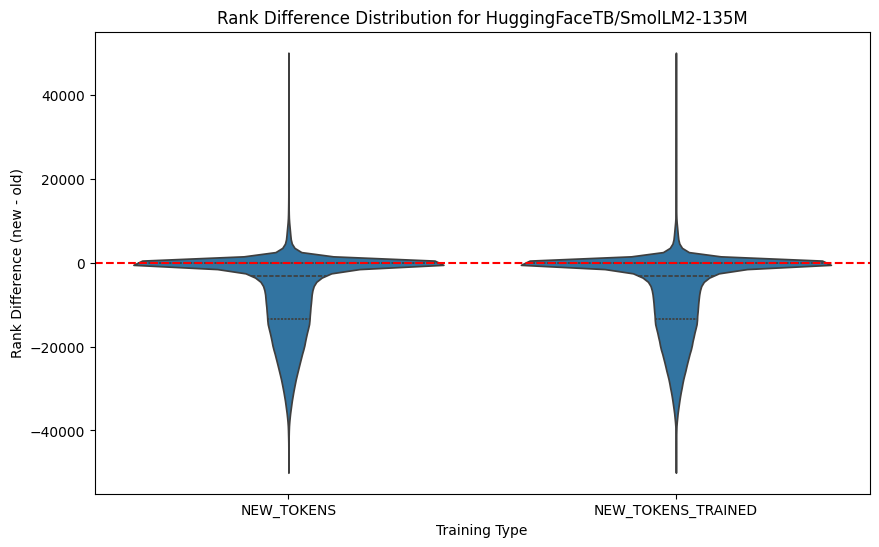
\includegraphics[width=1\textwidth]{Figures/rank_diff_dist_violin.png}
    \caption{Distribution of rank differences across the entire results data. Negative numbers show preference towards \texttt{new\_token}.}
    \label{fig:violin_rank_dist}
\end{figure}
This result provides a mechanistic explanation for why vocabulary adaptation can improve fluency in sampling-based generation: even if benchmark accuracy remains unchanged, the model shows a latent preference for producing new tokens, which may lead to more natural completions during free-form generation.\unsure{add Annex plots for all the other Models and "Number New Tokens"}
 


\subsection{Retained Performance on Source Language}

While our primary interest is in Portuguese adaptation, it is equally important to verify that modifications do not degrade performance in the model’s original training language(s). To this end, we evaluated all variants on the \textbf{Massive Multitask Language Understanding (MMLU)} benchmark, which covers 57 academic subjects and serves as a broad proxy for general knowledge and reasoning ability.

Table~\ref{tab:mmlu-results} reports MMLU accuracy for each configuration.

\begin{table}[h]
\centering
\begin{tabular}{lccc}
\hline
\textbf{Model} & \textbf{New Tokens} & \textbf{Type} & \textbf{MMLU (\%)} \\
\hline
SmolLM2-135M   & 0     & Baseline      & 23.25 \\
SmolLM2-135M   & 1000  & No Training   & 23.25 \\
SmolLM2-135M   & 1000  & With Training & 23.25 \\
SmolLM2-135M   & 5000  & No Training   & 23.25 \\
SmolLM2-135M   & 5000  & With Training & 23.25 \\
SmolLM2-135M   & 7500  & No Training   & 23.25 \\
SmolLM2-135M   & 7500  & With Training & 23.25 \\
\hline
SmolLM3-3B     & 0     & Baseline      & 56.67 \\
SmolLM3-3B     & 1000  & No Training   & 56.67 \\
SmolLM3-3B     & 1000  & With Training & 56.67 \\
SmolLM3-3B     & 5000  & No Training   & 56.67 \\
SmolLM3-3B     & 5000  & With Training & 56.67 \\
SmolLM3-3B     & 7500  & No Training   & 56.67 \\
SmolLM3-3B     & 7500  & With Training & 56.67 \\
\hline
Qwen2.5-1.-Instruct   & 0     & Baseline      & 58.97 \\
Qwen2.5-1.5B-Instruct   & 1000  & No Training   & 58.97 \\
Qwen2.5-1.5B-Instruct   & 1000  & With Training & 58.97 \\
Qwen2.5-1.5B-Instruct   & 5000  & No Training   & 58.97 \\
Qwen2.5-1.5B-Instruct   & 5000  & With Training & 58.97 \\
Qwen2.5-1.5B-Instruct   & 7500  & No Training   & 58.97 \\
Qwen2.5-1.5B-Instruct   & 7500  & With Training & 58.97 \\
\hline
\end{tabular}
\caption{MMLU accuracy (baseline vs. adapted tokenizers).}
\label{tab:mmlu-results}
\end{table}

Results demonstrate that MMLU performance is \textbf{completely stable} across all settings. This indicates that tokenizer adaptation does not interfere with the model’s original linguistic or reasoning capabilities. In other words, improvements for Portuguese are not obtained at the expense of performance in the source language.


\subsection{Observations}
Overall, benchmark scores showed minor improvements after token adaptation, although these gains were only marginal. Generation efficiency, however, showed promising results, specifically with the smaller single-language model. These improvements suggest that token adaptation alone does not guarantee downstream task improvements, but may create the representational conditions for further fine-tuning gains.


\section{Qualitative Analysis}

While benchmark accuracy provides a coarse view of task performance, it does not fully capture how adapted models \textit{feel} when generating text. To complement quantitative metrics, we conducted a qualitative evaluation of model completions along two dimensions that reflect different aspects of cross-lingual adaptation:  
\textbf{(i) Syntactic Fluency}, i.e., whether outputs form well-structured sentences with plausible morphology and word order; and
\textbf{(ii) Semantic Grounding}, i.e., whether outputs remain on-topic and respect the intended meaning of prompts. 

These dimensions map directly to the linguistic challenges of adapting a model trained in one language for use in another: respecting syntax, grounding new embeddings in meaning, and producing stylistically natural text.

All results presented bellow were obtained with the following configuration:
\begin{itemize}
    \item \textbf{Model: } \texttt{HuggingFaceTB/SmolLM2-135M}\footnote{SmolLM2-135M source - \href{https://huggingface.co/HuggingFaceTB/SmolLM2-135M}{link}}
    \item $temperature$\footnote{Temperature scales the logits before sampling; higher values encourage more diverse but less predictable generations.}$ = 0.8$;
    \item $top\_p$\footnote{Nucleus sampling parameter; tokens are sampled from the smallest probability mass $p \geq 0.9$, balancing relevance with diversity.}$ = 0.9$;
    \item $top\_k$\footnote{Sampling restricted to the $k=100$ most likely tokens, removing low-probability candidates.}$ = 100$.  
\end{itemize}

\subsection*{Illustrative Examples}

\begin{table}[h]
\centering
\begin{tabular}{p{\linewidth}}
\toprule
\textbf{Prompt:} \prompt{"Para calcular a raiz quadrada de um número manualmente,"} \\
\midrule
\begin{tabularx}{\linewidth}{p{0.33\linewidth}|p{0.33\linewidth}|p{0.33\linewidth}}
\textbf{Baseline} & \textbf{Adapted w/ 5000 tokens} & \textbf{Adapted and Trained} \\
\generation{"retorna uma posição. python x = 10 y = 20 print(f"A raiz quadrada de \{x\} e \{y\} é \{x ** "} & \generation{"utilizando o tipo de cálculo de fatorial. Por exemplo, se uma quantidade de pemares a pouco mais de um alcance, seja 110000"} & \generation{"e construa um número quadrado em duas partes aixa e a linda, A matoê estra: A matoê do primeiro num méênico da raiz"} \\
\end{tabularx} \\
\midrule
\textbf{Prompt:} \prompt{"Nos dias de hoje, democracia é o sistema politico"} \\
\midrule
\begin{tabularx}{\linewidth}{p{0.33\linewidth}|p{0.33\linewidth}|p{0.33\linewidth}}
\textbf{Baseline} & \textbf{Adapted w/ 5000 tokens} & \textbf{Adapted and Trained} \\
\generation{". Ao demorar por 6 dias para que seja o seu emissar, a dor da elemência eleitora atual aumentará e o próprio p"} & \generation{"que ele, na quais seriam a diferença, de forma fatoriva, de uma média de 013020 00010000000010..."} & \generation{", o que não se encontra nis. A que também é o democracia. EIuão de Hic e da Cria de Io Paulo. Hic"} \\
\end{tabularx} \\
\midrule
\textbf{Prompt:} \prompt{"O poema seguinte contém várias palavras-chave: azul, borboleta e sol:"} \\
\midrule
\begin{tabularx}{\linewidth}{p{0.33\linewidth}|p{0.33\linewidth}|p{0.33\linewidth}}
\textbf{Baseline} & \textbf{Adapted w/ 5000 tokens} & \textbf{Adapted and Trained} \\
\generation{"e sí, e também, e física e próximo. O poema também tem como seu último último, o estudante d"} & \generation{"céu de la tierra, y vrgosos deixa. Vídeo como nome: «Cicio-dei alcoba e sol», com aumos dos dcimentoimens"} & \generation{"Este estará por esqueço da esquina do lado do que a leitura seja frente ao largo do espaço”. Para outras palavras-chave,"} \\
\end{tabularx} \\
\bottomrule
\end{tabular}
\caption{Illustrative Examples of Model Completions (Baseline vs. Adapted vs. Adapted and Trained)}
\label{tab:example_completions_horizontal}
\end{table}




\subsection*{Observations}
\begin{itemize}
    \item \textbf{Syntactic Fluency:} The baseline often produced truncated or incomplete sentences. Adapted+trained variants showed more fluent structures, though sometimes with invented morphology (e.g., ``matoê'') or undecodable symbols.
    \item \textbf{Semantic Grounding:} For mathematical prompts, adapted models drifted into nonsensical placeholders, reflecting weak grounding of numerical concepts. In political and poetic prompts, however, the adapted+trained model produced more topically aligned continuations, showing partial semantic integration of new tokens.
\end{itemize}


% \subsection*{Scorecard Summary}
% To synthesize these observations, we manually annotated each system variant with a coarse qualitative rating across the three dimensions (S = satisfactory, P = partial, U = unsatisfactory). This scale is intentionally coarse and intended for exploratory comparison rather than definitive evaluation.

% \begin{table}[h]
% \centering
% \begin{tabular}{lccc}
% \hline
%  & \textbf{Syntactic Fluency} & \textbf{Semantic Grounding} \\
% \hline
% Baseline & U & U \\
% Adapted (5k) & P & U \\
% Adapted+Trained & P & U \\
% \hline
% \end{tabular}
% \caption{Qualitative ratings of completions (manual annotation).}
% \label{tab:qualitative_scorecard}
% \end{table}


\subsection*{Limitations}
As with the quantitative evaluation, these qualitative findings must be interpreted in light of model constraints. The analysis was conducted on \texttt{HuggingFaceTB/SmolLM2-135M}, a small (135M parameter) model trained exclusively in English. These conditions amplify failure modes such as truncation, invented morphology, and weak semantic grounding, making improvements more difficult to observe. Consequently, the qualitative evaluation should be seen as a proof-of-concept rather than a definitive test of the approach. Future work (see Chapter~\ref{chap:conclusions}) should evaluate wider spectrum of model architectures.





\section{Discussion}
Our results reveal that:
\begin{itemize}
    \item Accuracy on PT-PT benchmarks remains largely unchanged by vocabulary expansion alone.
    \item Efficiency gains are achievable for smaller models but not guaranteed for larger multilingual ones.
    \item Qualitative effects depend strongly on model architecture and may require further fine-tuning to stabilize.
\end{itemize}

This supports our thesis hypothesis that tokenizer adaptation can make small, resource-efficient models more suitable for underrepresented languages like European Portuguese, but highlights the limitations of applying the same strategy universally.














%%%%%%% ----> OLD CHAPTER
% % Chapter Template

% % Main chapter title
% \chapter{Results}

% % Short version of the title for the header
% \chaptermark{Results}

% % Chapter Label
% \label{chap:results}

% This chapter presents the experimental results of our tokenizer adaptation method. As discussed in Chapter~\ref{Section3}, we evaluate performance using two established benchmarks for European Portuguese: \textbf{CalamePT} (§\ref{subsec:dataset-calamept}), which measures text completion, and \textbf{SuperGluePTPT} (§\ref{subsec:dataset-superglueptpt}), which evaluates reasoning and comprehension. In addition, we introduce a custom efficiency metric (\S\ref{sec:gen_efficiency}) to assess the impact of tokenizer modifications on token usage during generation.


% \section{Evaluation Methodology}
% All evaluations follow the benchmark-specific protocols described in Chapter~\ref{Section3}. For clarity:

% \begin{itemize}
%     \item \textbf{CalamePT:} Accuracy is measured as the proportion of correctly predicted final words in incomplete Portuguese phrases.
%     \item \textbf{SuperGluePTPT (BoolQ-PT):} Accuracy is measured as the proportion of correct yes/no answers in the binary classification task.
% \end{itemize}

% We compare baseline models against variants adapted with (i) added tokens only and (ii) added tokens followed by lightweight embedding training. 

% \subsection{CalamePT Benchmark}
% The CalamePT benchmark evaluates a model's ability to perform contextually appropriate text completion. It comprises 2,476 phrases, including 406 handwritten phrases and 2,070 phrases automatically generated using GPT-3.5, each designed such that the final word can be logically predicted from the preceding context.

% A representative example from this benchmark is: "Ela correu durante horas para alcançar a linha de \textunderscore{chegada}" (She ran for hours to reach the finish line), where "chegada" (finish) is the target completion token.

% The evaluation protocol is as follows:
% \begin{enumerate}
%     \item The model receives the text with the final word omitted as input
%     \item If the first word generated by the model matches the expected completion word, a positive score is assigned
%     \item This process is repeated across all prompts in the dataset
%     \item The final score represents the percentage of correctly completed prompts
% \end{enumerate}

% This methodology provides a direct assessment of the model's ability to understand and generate contextually appropriate Portuguese vocabulary.

% \subsection{SuperGluePTPT Benchmark}
% The SuperGluePTPT dataset was developed through an automated translation of the original English SuperGlue benchmark \cite{https://proceedings.neurips.cc/paper/2019/hash/4496bf24afe7fab6f046bf4923da8de6-Abstract.html} into European Portuguese using \cite{DeepL}\unsure{add references}.

% This benchmark focuses on evaluating higher-level language understanding through a series of binary classification tasks. The evaluation methodology involves:

% \begin{enumerate}
%     \item Presenting the model with questions that require yes/no responses
%     \item Employing specific prompt engineering techniques to constrain model outputs to binary responses
%     \item Calculating accuracy as the percentage of correct answers relative to the ground truth
% \end{enumerate}

% This approach provides insight into the model's capacity for complex reasoning and language understanding in Portuguese, beyond simple token prediction.

% \section{Results Analysis}
% \subsection{Comparative Performance}
% The adapted model demonstrated slight improvements in Portuguese language processing capabilities compared to the baseline model. Table \ref{tab:benchmark_results} presents a comparative analysis of performance across both evaluation benchmarks.

% \begin{table}[h]
% \centering
% \caption{Performance Comparison on Portuguese Language Benchmarks}
% \label{tab:benchmark_results}
% \begin{tabular}{lcccc}
% \hline
% \textbf{Model} & \textbf{Added Tokens} & \textbf{Type} & \textbf{CalamePT (\%)} & \textbf{SuperGluePTPT (\%)} \\
% \hline
% SmolLM2-135M & 0     & Baseline                  & 13.63\% & 1.44\% \\
% \toprule[0.5pt]
% SmolLM2-135M & 1000  & No Training & 13.63\% & 1.44\% \\
% SmolLM2-135M & 5000  & No Training & 13.63\% & 1.45\% \\
% SmolLM2-135M & 10000 & No Training & 13.63\% & 1.45\% \\
% \midrule[0.5pt]
% SmolLM2-135M & 1000  & With Training & 13.63\% & 1.44\% \\
% SmolLM2-135M & 5000  & With Training & 13.63\% & 1.45\% \\
% SmolLM2-135M & 10000 & With Training & 13.63\% & 1.45\% \\
% \midrule[1.5pt]
% Qwen2.5-1.5B & 0     & Baseline      & 49.81\% & 40.20\% \\
% \midrule[0.5pt]
% Qwen2.5-1.5B & 1000  & No Training & 49.81\% & 39.82\% \\
% Qwen2.5-1.5B & 5000  & No Training & 49.81\% & 40.05\% \\
% Qwen2.5-1.5B & 10000 & No Training & 49.76\% & 40.06\% \\
% \midrule[0.5pt]
% Qwen2.5-1.5B & 1000  & With Training & 49.81\% & 39.78\% \\
% Qwen2.5-1.5B & 5000  & With Training & 49.81\% & 40.01\% \\
% Qwen2.5-1.5B & 10000 & With Training & 49.76\% & 40.02\% \\
% \bottomrule[1.5pt]
% \end{tabular}
% \end{table}

% \subsection{Generation Efficiency Analysis}
% One of the key results we aimed for in our tokenizer adaptation was generation efficiency, measured by the Fertility Output metric. This metric quantifies the number of output tokens required to generate a single meaningful word in Portuguese. Figure \ref{fig:token_efficiency}\unsure{ADD figure showing evolution of fertility Output} illustrates the comparative generation efficiency between the original and adapted models.

% Our analysis of the Fertility Output metric revealed interesting patterns in generation efficiency across different models:

% \begin{itemize}
%     \item \textbf{SmolLM2-135M Baseline}: 3.07 tokens per generated word (average)
%     \item \textbf{SmolLM2-135M with 7,500 new tokens}: 2.86 tokens per generated word (average)
%     \item \textbf{Qwen2.5-1.5B Baseline}: 1.74 tokens per generated word (average)
%     \item \textbf{Qwen2.5-1.5B with 7,500 new tokens}: 2.17 tokens per generated word (average)
% \end{itemize}

% Interestingly, the results show a model-dependent effect. The smaller monolingual SmolLM2-135M model showed a 6.8\% improvement in generation efficiency with the adapted tokenizer, requiring fewer tokens to generate Portuguese words. However, the larger multilingual Qwen2.5-1.5B model exhibited a 24.7\% decrease in generation efficiency, requiring more tokens to generate words after adaptation.\unsure{This section may be updated with results from additional models (monolingual large models and multilingual small models) to better understand the factors affecting generation efficiency.}

% This contrasting behavior suggests that the relationship between tokenization adaptation and generation efficiency is complex and model-dependent.\unsure{Further analysis with different model architectures may provide more insights into this relationship.} The improvement observed in the smaller model indicates that our approach can enhance generation efficiency for certain model architectures, which could be particularly beneficial for applications where generation speed and resource efficiency are important considerations.

% The improvement in generation efficiency for the SmolLM2-135M model can be particularly significant for applications requiring real-time text generation, where the cumulative effect can substantially impact the model's responsiveness and resource utilization.\unsure{Additional testing with other monolingual models of different sizes would help confirm if this benefit extends to other architectures.}

% \subsection{Qualitative Analysis}
% To complement our quantitative metrics, we conducted a qualitative analysis of model outputs before and after tokenizer adaptation. This analysis focused on three key aspects of language generation:

% \begin{itemize}
%     \item \textbf{Grammatical Accuracy}: PLACEHOLDER FOR RESULTS REGARDING GRAMMATICAL ACCURACY
    
%     \item \textbf{Semantic Coherence}: PLACEHOLDER FOR RESULTS REGARDING SEMANTIC COHERENCE
    
%     \item \textbf{Cultural References}: PLACEHOLDER FOR RESULTS REGARDING CULTURAL KNOWLEDGE
% \end{itemize}

% Table \ref{tab:example_completions} provides illustrative examples of completions generated by the baseline and adapted models for the same prompts, highlighting the qualitative improvements achieved through tokenizer adaptation.

% \begin{table}[h]
% \centering
% \caption{Example Completions from Baseline and Adapted Models}
% \label{tab:example_completions}
% \begin{tabular}{p{4cm}p{5cm}p{5cm}}
% \hline
% \textbf{Prompt} & \textbf{Baseline Model} & \textbf{Position-Weighted Model} \\
% \hline
% POPULATE THIS TABLE WITH VALUES & This is a sample completion from the baseline model. & This is a sample completion from the position-weighted model. \\
% \hline
% \end{tabular}
% \end{table}

% These observations suggest that the tokenizer adaptation approach can be both effective and deffective, dependent on the model architecture. While the adapted tokenizer successfully reduces the number of tokens required to encode Portuguese text in smaller monolingual models, larger or multilingual \unsure{edit once tests have been done on smaller multilingual and larger monolingual models} models won't benefit from the explored adaptation.

% The qualitative analysis further suggests that ...\unsure{populate once qualitative analysis has been executed}